% try to make flow chart more like diagrams in android book

\documentclass{article}
\usepackage[utf8]{inputenc}
\usepackage{tikz}
\usepackage{pgfplots}
\usetikzlibrary{shapes.multipart}
\usetikzlibrary{shapes.geometric, arrows}

\tikzstyle{activity} = [rectangle, rounded corners, minimum width=3cm, minimum height=1cm,text centered, draw=black, fill=green!30]

\tikzstyle{view} = [rectangle, rounded corners, minimum width=1cm, minimum height=1cm, text centered,  draw=black, fill=blue!30] 

\tikzstyle{process} = [rectangle, rounded corners, minimum width=3cm, minimum height=1cm, text centered, text width=3cm, draw=black,
fill=orange!30]

\tikzstyle{service} = [rectangle, rounded corners, minimum width=3cm, minimum height=1cm, text centered, text width=4cm, draw=black,
fill=red!30]

 \tikzstyle{class} = [rectangle split, rectangle split parts=2, rounded corners, minimum width=3cm, minimum
 height=1cm, text width=3cm, draw=black, text centered,
 fill=brown!30] 

 \tikzstyle{enum} = [rectangle split, rectangle split parts=2, rounded corners, minimum width=3cm, minimum
 height=1cm, text width=3cm, draw=black, text centered,
 fill=purple!40] 

 \tikzstyle{fragment} = [rectangle split, rectangle split parts=2, rounded corners, minimum width=3cm, minimum height=1cm, text width=3cm, draw=black,
 fill=black!30!green] 

\tikzstyle{arrow} = [thick,->,>=stealth]

% for the legend
% argument #1: any optviewns
\newenvironment{customlegend}[1][]{%
    \begingroup
    % inits/clears the lists (which might be populated from prevviewus
    % axes):
    \csname pgfplots@init@cleared@structures\endcsname
    \pgfplotsset{#1}%
}{%
    % draws the legend:
    \csname pgfplots@createlegend\endcsname
    \endgroup
}%

% makes \addlegendimage available (typically only available within an
% axis environment):
\def\addlegendimage{\csname pgfplots@addlegendimage\endcsname}


\begin{document}

\begin{tikzpicture}[node distance=2cm]

\node (main) [activity]                                     {MainActivity.java};
\node (BLE) [service, left of=main, xshift=-4cm, yshift=-1cm]{BluetoothLeService.java};

\node (DA) [activity, below of=main]                          {DeviceActivity.java};
\node (plot) [view, right of=DA, xshift=3.5cm]             {plot.xml};

\node (HP) [activity, below of=DA]                            {HistoryPlot.java};
\node (history) [view, below of=HP]                        {history.xml};

\node (VPA) [activity, left of=HP, xshift=-4cm]               {ViewPagerActivity.java};
\node (fragpage) [view, below of=VPA]                      {fragment\_pager.xml}; 

\node (sensor) [class, below of=fragpage,yshift=-1cm] {Sensor.java 
\nodepart[align=left]{second} Accelerometer\{ \\ convert(RawData)\} \vspace{1 mm}\\ Gyroscope\{ \\convert(RawData)\}};

\node (point3d) [class, right of=sensor,xshift=3cm] {Point3D.java 
\nodepart[align=left]{second} double x \\ double y \\ double z};

\node (scanview) [fragment, right of=point3d,xshift=3cm] {ScanView.java \nodepart{second} null};

\node (fragscan) [view, below of=scanview] {fragment\_scan.xml};
\node (svpic) [below of=fragscan,yshift=-1.5cm] {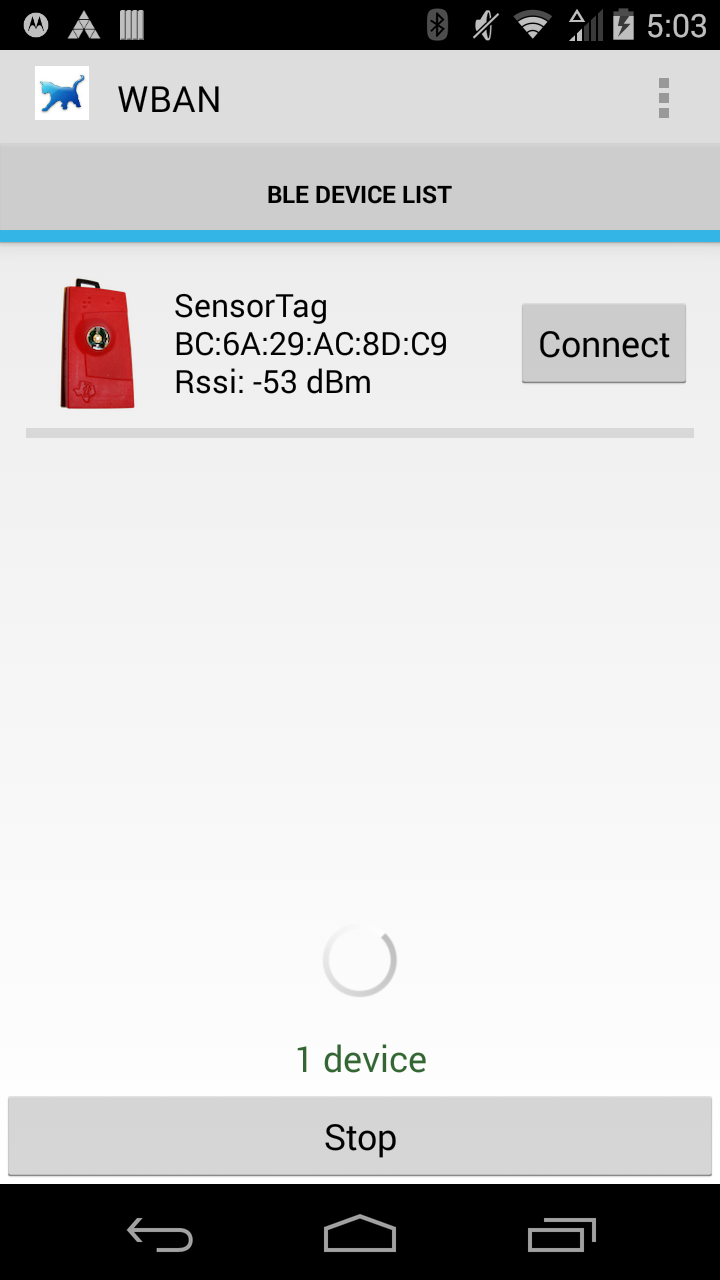
\includegraphics[width=3cm]{pics/device_found.png}};

%\node (point3d) []

%% main to *
\draw [arrow] (main) to [bend right=20] node[anchor=west] {fragment} (VPA); 
\draw [arrow] (main) -- (DA);
\draw [arrow] (main) to [bend right=10] node[anchor=east] {startService()} (BLE);

% DA to * 
\draw [arrow] (DA) -- node[anchor=east] {startActivity()} (HP);
\draw [arrow] (DA) -- node[anchor=south] {setContentView()} (plot);

\draw [arrow] (HP) -- node[anchor=east] {setContentView()} (history);

\draw [arrow] (VPA) -- node[anchor=east] {setContentView()} (fragpage);

%%% second legend
%%% http://tex.stackexchange.com/questviewns/54794/using-a-pgfplots-style-legend-in-a-plain-old-tikzpicture 

\begin{customlegend}[legend entries={Activity,View,Class,Fragment,Service}, legend style={at={(5,0.5)},anchor=center}]
  \addlegendimage{black,fill=green!30,area legend}
  \addlegendimage{black,fill=blue!30,area legend}
  \addlegendimage{black,fill=brown!30,area legend}
  \addlegendimage{black,fill=black!30!green,area legend}
  \addlegendimage{black,fill=red!30,area legend}

\end{customlegend}

\end{tikzpicture}

\end{document}